\begin{center}
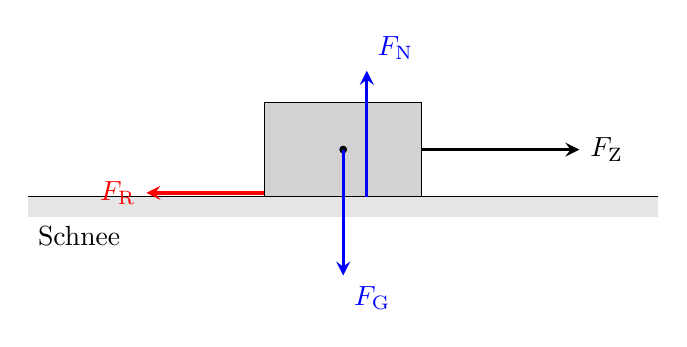
\begin{tikzpicture}[>=stealth]
 \fill[gray!20] (-4,0) rectangle (4,-0.25);
 \draw (-4,0) -- (4,0);
 \node[anchor=north west] at (-4,-0.25) {Schnee};
 \draw[fill=gray!35] (-1,0) rectangle (1,1.2);
 \fill (0,0.6) circle (0.05);
 \draw[->, very thick] (1,0.6) -- ++(2.0,0) node[right] {$F_\mathrm{Z}$};
 \draw[->, very thick, red] (-1,0.05) -- ++(-1.5,0) node[left] {$F_\mathrm{R}$};
 \draw[->, very thick, blue] (0,0.6) -- ++(0,-1.6) node[anchor=north west] {$F_\mathrm{G}$};
 \draw[->, very thick, blue] (0.3,0) -- ++(0,1.6) node[anchor=south west] {$F_\mathrm{N}$};
\end{tikzpicture}
\end{center}

Die Skifahrerin gleitet mit konstanter Geschwindigkeit, die resultierende Kraft auf sie ist null. Zieht der Lift parallel zur Schneefläche, ist seine Zugkraft gleich der Gleitreibungskraft $\mu_\mathrm{G}\,m\,g$. Geschwindigkeit und Länge der Strecke spielen keine Rolle.

Für Ski auf Schnee gibt FoTaBe (S.~189) $\mu_\mathrm{G} = \muGO \pm \dmuO$. Am kleinsten ist die Zugkraft bei der kleinsten Reibungszahl $\mu_\mathrm{min} = \mumin$:
\begin{align}
 F_\mathrm{Z} &= \FZuF \\
   &= \mumin\cdot\mSk\cdot\gE \\
   &= \FZu \approx \result{\FZuP{0}{2}}
\end{align}
Mit dem typischen Wert $\mu_\mathrm{G} = \muGO$ wären es $\FZtP{0}{2}$.
